\section{Introduction}
\label{sec:intro}

A diffusion model generates by reversing a noising process, and the reversal is driven by
the score $\score(\vx,t)=\nabla_{\vx}\log\Pt(\vx)$ of the noised data law
\citep{sohl2015deep,ho2020denoising,song2021scorebased}. Training regresses a network onto
that score through denoising \citep{vincent2011connection}, so every question about what the
network has learned is a question about the distance between what it computes and the score
it should have computed. For real data that target is unknown: a large error cannot be told
from a hard target, and the solvable alternatives are Gaussian, whose scores are linear, or
mixtures, whose nonlinearity lives in a discrete label rather than in any dependence between
coordinates.

\paragraph{The structural thesis: learn the local law, infer globally.}
Data with a one-dimensional dependence structure sit between those cases. If the clean
sequence is a first-order Markov chain with transition kernel $\kernel(a'\mid a)$, then under
coordinatewise Gaussian noising the posterior factor graph is a tree, the score is a
posterior mean (Tweedie's identity), and one forward--backward sweep of belief propagation (BP)
returns it exactly for \emph{any} continuous kernel, including those whose score has no
closed form (\cref{sec:inference}). A network that denoises such data must learn the
composition of local transitions into a global posterior from examples. The structured
estimator learns only the local law and delegates the composition to an exact algorithm. When the
kernel is unknown it is learned from noised sequences alone by expectation--maximisation
(EM) around the same sweep (\cref{sec:learning}); the result, EM--BP, is the paper's
estimator (\cref{fig:summary}).

\begin{figure*}[t]
  \centering
  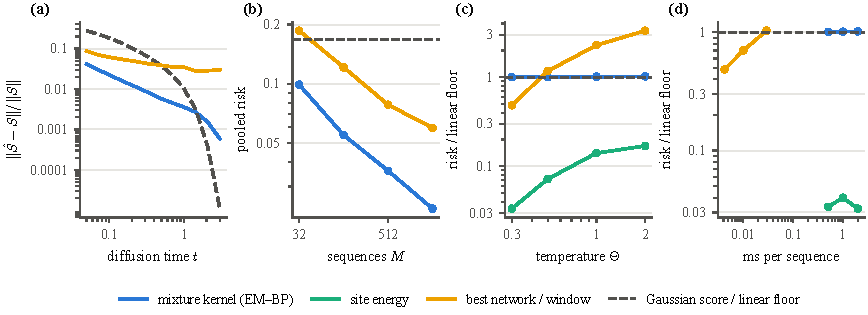
\includegraphics[width=\textwidth]{ff-summary.pdf}
  \caption{\textbf{Summary.} Relative score error against the exact score, pooled over a
  twelve-level noise schedule. (a)~Per-level error on the linear chain with Laplace noise
  ($\nseq=2048$ training sequences): the learned kernel (blue) beats the best network (yellow)
  at every level and the Gaussian score (dashed) except at the highest noise levels.
  (b)~Pooled error against the number of training sequences on the same chain.
  (c)~The $\phi^4$ field ($\nseq=2048$): risk divided by the linear (Gaussian) floor against
  temperature $\Temp$; the five-parameter site energy (green) is far below it, the linear-drift
  mixture kernel of (a, b) sits on it, and the window network rises above it when the field is hot.
  (d)~The same ratio against inference time on three lattice spacings at $\Temp=0.3$ (eight
  threads, the largest network variants).}
  \label{fig:summary}
\end{figure*}

\paragraph{Two laboratories with exact scores.}
The framework is stated for a general kernel (\cref{sec:setup}); we test it on two concrete
cases chosen because their scores can be computed exactly and compared with everything else.
The first is a linear chain with non-Gaussian driving noise, whose covariance is fixed by two
numbers and whose shape by the noise law, so Gaussian, Laplace, Student-$t$, uniform and
bimodal noise share one covariance exactly and differ only in higher-order structure; it
separates, by construction, what diffusion noise does to correlation from what it does to
shape (\cref{sec:experiments}). The second is the one-dimensional $\phi^4$ field, the
stochastic Allen--Cahn model, whose lattice snapshots are exactly Markov, whose kernel is
nonlinear (a double well with domains and kinks), and which has a physical vocabulary
(temperature, correlation length, kink density) and exact transfer-matrix references
(\cref{sec:field}).

\paragraph{Contributions.}
\begin{enumerate}[label=(\roman*),leftmargin=1.6em,itemsep=0.1em,topsep=0.2em]
\item \emph{Exact denoising for any Markov kernel.} Score estimation for Markov data reduces
to posterior means, which BP computes exactly up to a quadrature we measure
(\cref{sec:inference}); the Gaussian kernel is a clean sanity check, since BP with Gaussian
messages is the linear score and the Kalman smoother (\cref{prop:lmmse,prop:kalman};
\cref{sec:sanity}).
\item \emph{The kernel is learnable from noise, and learning it works.} EM through the same
sweep recovers the kernel from one noised view per sequence (\cref{sec:learning}). With a kernel of
a few parameters it beats the neural denoisers it is compared with (six on the linear chain, two on the field) at every sample
size, by a paired factor $\matchedRatioBestD$ at EM--BP's own information interface on the linear chain and by
$\fldNetRatioMin$--$\fldNetRatioMax$ on the field (the best network over the site energy at $\nseq=2048$).
\item \emph{The kernel family is the real modelling choice.} The linear-drift mixture is
exactly right for the linear chain and sits on the linear floor on the field; the
five-parameter site energy, the physicist's pair energy, is best on every field cell; an
unrestricted or neural kernel earns its parameters only where the simple family is
misspecified (\cref{sec:field,sec:limits}).
\item \emph{Cost and limits, measured.} BP is slower per sequence than a network; a coarser grid
recovers most of the gap for the field kernels, and a Fourier representation of the messages
is not worth building (\cref{sec:compute}). A latent shared by a whole sequence leaves a bias
that no sample size removes, which augmenting the state repairs (\cref{sec:limits}).
\end{enumerate}

\paragraph{Supporting theory: what noise erases.}
Why structure matters most where the noise has not yet erased it is a general fact about the
Ornstein--Uhlenbeck channel, and we prove it in the laboratory where it can be checked: the
channel attenuates the Hermite moment of degree $m$ by $e^{-mt}$ exactly, so the Fisher
information a noised sequence carries about a feature first visible at degree $m$ decays as
$e^{-2mt}$ with an explicit constant (correlation as $e^{-4t}$, non-Gaussian shape as $e^{-8t}$),
and the gap between the true score and that of the covariance-matched Gaussian is
$\tfrac16\lVert\kappa_4\rVert_F^2e^{-8t}$ (\cref{sec:theory}). We treat this as supporting
rather than central: it explains where the structured estimator gains, not why it is exact.
